\documentclass[11pt,a4paper]{report}

%
% Packages
%
\usepackage[T1]{fontenc}
\usepackage[utf8]{inputenc}
\usepackage{amsmath,amsthm,amssymb}
\usepackage[svgnames]{xcolor}
\usepackage[english,french]{babel}
\usepackage{multicol}
\usepackage{pstricks,pst-node,pst-text,pst-poly,pst-3d}
\usepackage{enumitem}
\usepackage{sidenotes}
\usepackage{graphicx} % Required to insert images
\usepackage{array}
\usepackage{booktabs} % Required for better horizontal rules in tables


%
% Constant and Variables
%
\setlength{\textwidth}{175mm}
\setlength{\textheight}{255mm}
\setlength{\oddsidemargin}{-10mm}
\setlength{\topmargin}{-15mm}
\setlength{\parskip}{0.2cm}

\definecolor{vertfonce}{rgb}{0,0.5,0}

%
% Commands
%
\newcommand{\ds}{\displaystyle}
\newcommand{\scr}{\scriptscriptstyle}
\newcommand{\bs}[1]{\ensuremath{\boldsymbol{#1}}}
\renewcommand{\leq}{\leqslant}
\newenvironment{refer} 
{
	\begin{list}
		{}
		{
			\setlength{\labelwidth}{.5em}
			\setlength{\leftmargin}{0.4cm}
			\setlength{\itemsep}{0cm}
		} 
	}
	{\end{list}}
%\pagenumbering{roman}
%\setcounter{page}{1}

%
\newcounter{num}
\newcommand{\exo}{\addtocounter{num}{1}\noindent{\bf{Exercice \thenum}}\\[-1mm]}
%

%
\newcommand{\donnee}[1]{\\{Donnée: } \emph{#1}}
%


%
% Math
%
\newcommand{\Real}{\mathbb R}
\newcommand{\RPlus}{\Real^{+}}
\newcommand{\norm}[1]{\left\Vert#1\right\Vert}
\newcommand{\abs}[1]{\left\vert#1\right\vert}
\newcommand{\setn}[1]{\left\{#1\right\}_{\scriptscriptstyle n \ge 1}}
\newcommand{\set}[1]{\left\{#1\right\}}
\newcommand{\seq}[1]{\left<#1\right>}
\newcommand{\eps}{\varepsilon}
\newcommand{\To}{\longrightarrow}
\newcommand{\Prob}{\rm{P}}
\newcommand{\F}{\mathcal{F}}
\newcommand{\h}{\mathcal{H}}
\newcommand{\M}{\mathcal{M}}
\newcommand{\N}{\mathcal{N}}
\newcommand{\E}{{\rm E}}
\newcommand{\Hnull}{{\rm H}_{0}}
\newcommand{\Hone}{{\rm H}_{1}}
\newcommand{\Var}{{\rm Var}}
\newcommand{\Cov}{{\rm Cov}}
\newcommand{\sign}{{\rm sign}}
\newcommand{\med}{{\rm med}}
\newcommand{\tr}{{\rm tr}}
\newcommand{\T}{{\text{\tiny \rm T}}}
\newcommand{\minf}{- \, \infty}
\newcommand{\intervalle}[4]{\mathopen{#1}#2\mathpunct{},#3\mathclose{#4}}
\newcommand{\intervalleff}[2]{\intervalle{[}{#1}{#2}{]}}
\newcommand{\intervalleof}[2]{\intervalle{]}{#1}{#2}{]}}
\newcommand{\intervallefo}[2]{\intervalle{[}{#1}{#2}{[}}
\newcommand{\intervalleoo}[2]{\intervalle{]}{#1}{#2}{[}}   
%
\newcommand{\separation}{{\begin{center}\rule{10cm}{0.25pt}\end{center}}\noindent}
%
\frenchspacing

\graphicspath{ {./} }


\begin{document}
	\header{probabilités élémentaires}{Série 1}
	%
	% Exercice 1
	%
	\begin{exo}
		\donnee{Un groupe de consommateurs a réalisé une étude pour analyser le service offert par 200 employés de	divers restaurants. On s’intéresse à une possible relation entre la qualité du service et la qualification du personnel (diplômé d’une école hôtelière ou non). Les résultats de l’enquête figurent dans le tableau ci-dessous : 
			\begin{center}
				\begin{tabular}{lll}
					& Bon service & mauvais service \\
					\toprule
					Diplôme & 61 & 28 \\
					\midrule
					Sans diplôme & 30 & 81 \\
					\bottomrule
				\end{tabular}
			\end{center}}
		Rappel : $P(A) = \frac{\text{Nombre de cas favorables}}{\text{Nombre de cas possibles}}$
		\begin{subexo}{Calculer les probabilités d’avoir choisi une personne :}
		\begin{enumerate}[parsep=0cm, itemsep=3mm, topsep=3mm]
			\item dont le service est qualifié bon.
			\begin{enumerate}
				\item[ ] \text{Ici on réunis les bons services des personnes avec et sans diplôme. On a donc : } 
				\item[ ] \begin{center}{Cas fav.} = 61 + 30 = 91\end{center} 
				\item[ ] \text{Ensuite on calcul les cas possibles. On a donc : } 
				\item[ ] \begin{center}{Cas tot.} = 61 + 28 + 30 + 81 = 200\end{center} 
				\item[ ] \text{On applique la formule et on obtient : } 
				\item[ ] \begin{center}$\dfrac{91}{200} = 0,455$\end{center} 
			\end{enumerate}
			\item non diplômée.
			\begin{enumerate}
				\item[ ] \text{Ici on réunis les personnes sans diplôme, peut importe la qualité du service. On a donc : } 
				\item[ ] \begin{center}{Cas fav.} = 30 + 81 = 111\end{center} 
				\item[ ] \text{Ensuite on calcul les cas possibles. On a donc : } 
				\item[ ] \begin{center}{Cas tot.} = 61 + 28 + 30 + 81 = 200\end{center} 
				\item[ ] \text{On applique la formule et on obtient : } 
				\item[ ] \begin{center}$\dfrac{111}{200} = 0,555$\end{center} 
			\end{enumerate}
			\item diplômé dont le service est bon.
			\begin{enumerate}
				\item[ ] \text{Ici on réunis les personnes avec diplôme et une bonne qualité de service. On a donc : } 
				\item[ ] \begin{center}{Cas fav.} = 61\end{center} 
				\item[ ] \text{Ensuite on calcul les cas possibles. On a donc : } 
				\item[ ] \begin{center}{Cas tot.} = 61 + 28 + 30 + 81 = 200\end{center} 
				\item[ ] \text{On applique la formule et on obtient : } 
				\item[ ] \begin{center}$\dfrac{61}{200} = 0,305$\end{center} 
			\end{enumerate}
		\end{enumerate}
		\end{subexo}
		\begin{subexo}{Quelle hypothèse faites-vous pour déterminer ces probabilités ?}
			Toutes les probabilités sont \textbf{équiprobables}. C'est pour cela qu l'on peut utiliser la formule énnoncée dans les rappels de l'exercice.
			
		\end{subexo}
	\end{exo}
	%
	% Exercice 2
	%
	\begin{exo}
		\donnee{Sur le chemin de l’école, un étudiant de la HEIG–VD s’arrête toujours à la même station-service pour faire le plein d’essence. Il a constaté que les deux pompes de la station notées A et B ont la même probabilité d’être occupées. De plus, la probabilité que l’une des deux pompes au moins soit utilisée vaut 0.9 et celle que toutes les deux soient simultanément occupées est 0.5.}

		Pour faciliter la compréhension de cet exercice, on peut réaliser un diagramme de Venn.
		\begin{center}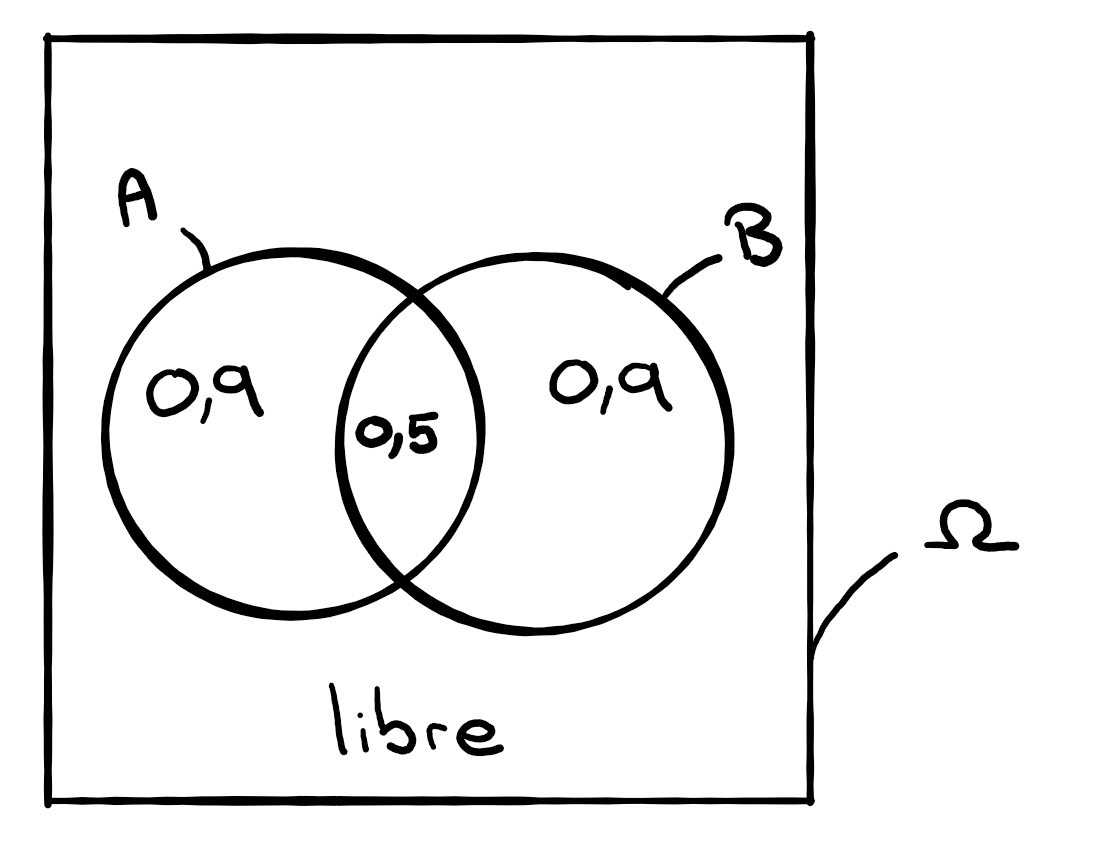
\includegraphics[scale=0.5]{ex2-diagrammeVenn}\end{center}
		Premièrement, posons que :
		\begin{multicols}{4}
			\begin{enumerate}[label=\alph*), parsep=0cm, itemsep=3mm, topsep=3mm]
				\item[ ] AO = La pompe A est occupée
				\item[ ] AL = La pompe A est libre
				\item[ ] BO = La pompe B est occupée
				\item[ ] BL = La pompe B est libre
			\end{enumerate}
		\end{multicols}
		\begin{center}$\Omega = \{(AL,BL),(AO,BL),(AL,BO),(AO,BO)\}$ \text{, évènements pas équiprobable !!!}\end{center}
		On sait que les probabilités que A soit libre sont les mêmes pour B. On note :
		\begin{center}$P(\{AL\}) = P(\{BL\})$\end{center}
		On sait aussi que :
		\begin{enumerate}
			\item[ ] $P(\text{au moins une pompe soite occupée}) = 0.9$
			\item[ ] $P(\text{les deux pompes soient occupées}) = 0.5$
			\item[ ] $P(\Omega) = 1$
		\end{enumerate}
		\begin{subexo}{Calculer la probabilité que les deux pompes soient disponibles.}
			Parmis les évènements probables on sait que : 
			\begin{center}$P\{(AO,BL),(AL,BO),(AO,BO)\} = 0.9$\end{center}
			Puisque nous cherchons la probabilité du couple manquant $(P\{(AL,BL)\})$, on pose :
			\begin{center}$P(\Omega) = P\{(AL,BL)\} + P\{(AO,BL),(AL,BO),(AO,BO)\}$\end{center}
			En remplaçant les probabilités connues par leurs valeurs, on obtient :
			\begin{center}$1 = P\{(AL,BL)\} + 0.9$\end{center}
			On peut donc en conclure que $P\{(AL,BL)\}  = 0.1$ et donc que la probabilité que la pompe A et B soient libre est de $0.1$
		\end{subexo}
	\end{exo}
	
	%
	% Exercice 3
	%
	\begin{exo}
		\donnee{df}
		\begin{multicols}{2}
			\begin{enumerate}[label=\alph*), parsep=1mm, itemsep=3mm, topsep=3mm]
				\item\label{q.quatrieme} $\left( \dfrac{5}{6} \right)^{10}$
				\item $1 - \left( \dfrac{5}{6} \right)^{10}$ 
			\end{enumerate}
		\end{multicols}
	\end{exo}
	
	%
	% Exercice 4
	%
	\begin{exo}
		\donnee{df}
		\begin{enumerate}[label=\alph*), parsep=0cm, itemsep=3mm, topsep=3mm]
			\item $P(A) = p$ \hspace{5mm} $P(B) = 2p$ \hspace{5mm} $P(A \cup B) = 0.28$
			\item $p = 0.1$
		\end{enumerate}
	\end{exo}
	
	%
	% Exercice 5
	%
	\begin{exo}
		\donnee{df}
		\begin{enumerate}[label=\alph*), parsep=0cm, itemsep=3mm, topsep=5mm]
			\item $0.49$
			\item $0.23$
		\end{enumerate}
	\end{exo}
	
	%
	% Footer
	%
	\vfill
	\hrule
	\vspace{2mm}
	\noindent {\tiny Corrigé Etudiant - TIC} \hfill {\tt \tiny \today}
\end{document}
